\chapter{Coordinate System and Vectors}\label{lec:lec16}
\definecolor{lightblue}{RGB}{173,216,230}
\begin{mdframed}[ backgroundcolor=lightblue, linewidth=1pt, hidealllines=true]
\section{Objectives}
By the end of this chapter, the you should be able to:
\begin{enumerate}[(i)]
	\item   To introduce the concept of coordinate systems and their importance in electromagnetism and antenna theory. 
	\item To explain the different types of \index{coordinate systems}coordinate systems, such as Cartesian, cylindrical, spherical, and others, and their properties, such as origin, axes, unit \index{vectors}.
	\item To demonstrate how to convert between different \index{coordinate systems} using transformation equations and matrices.
	\item To show how to perform basic operations, such as dot product, cross product, \index{gradient}, \index{divergence}, and index{curl}, on \index{scalar} and vector fields in different coordinate systems. 
	\item To apply the basic \index{coordinate system} operations to solve problems in electromagnetism and antenna theory.
	\item To enable understanding of the advantages and disadvantages of different coordinate systems for different applications in electromagnetism and antenna theory. 
	\item To develop the skills and intuition to choose the most appropriate coordinate system for a given problem or situation in electromagnetism and antenna theory. 
	\item To review and revise the mathematical background and tools needed to work with coordinate systems, such as trigonometry, calculus and linear algebra. 
	\item To provide examples and exercises that reinforce the learning outcomes and objectives of the coordinate system topic.
	
\end{enumerate}

\end{mdframed}

Up to this point, we have discussed one important case of transmission lines. We saw that when we brought in the concept of space, the voltage and current came to exist in the form of waves in the circuit. However, the concepts of voltage and current apply to \textbf{bound structures} like electrical circuits where you have conductors separated by dielectrics, coaxial cables, parallel wire transmission lines and so many others. In media that are \textbf{unbounded} or semi-infinite in extent or a media which is only di-electric, we find that the use of voltage and current is not very attractive. In fact, in many applications, it is very difficult to find quantities like voltage and current. In this situation, we have to go to the more fundamental quantities like the electric field and magnetic field. So having now got some feel for the wave phenomenon, especially for special cases like current and voltage, we depart to the more generalized phenomenon of electromagnetic waves and that is the waves in the form of electric and magnetic fields. Henceforth, we would discuss the phenomenon of electromagnetic waves in terms of electric field and magnetic field. Electric field and magnetic field are vector quantities so we have to deal with $\boldsymbol{E}$ and $\boldsymbol{H}$ analysis on three-dimensional space. To achieve this, we would revise our concept of vector calculus and vector algebra.

Let us first see how to represent the vector quantities in 3D space before going into vector algebra and calculus. Mathematically, we have to represent the quantities $\boldsymbol{E}$ and $\boldsymbol{H}$ as \index{vectors} in the three major coordinate systems.

\section{Coordinate systems}
The three major coordinate systems  used for vector representation in three-dimensional space are :
\begin{enumerate}[(i)]
\item Cartesian coordinate system ( x, y, z)
\item Cylindrical coordinate system ( r, $\phi$, z)
\item Spherical coordinate system (r,  $\theta$, $\phi$ )
\end{enumerate}

\subsection{Cartesian coordinate system}
\begin{figure}[h]
\centering
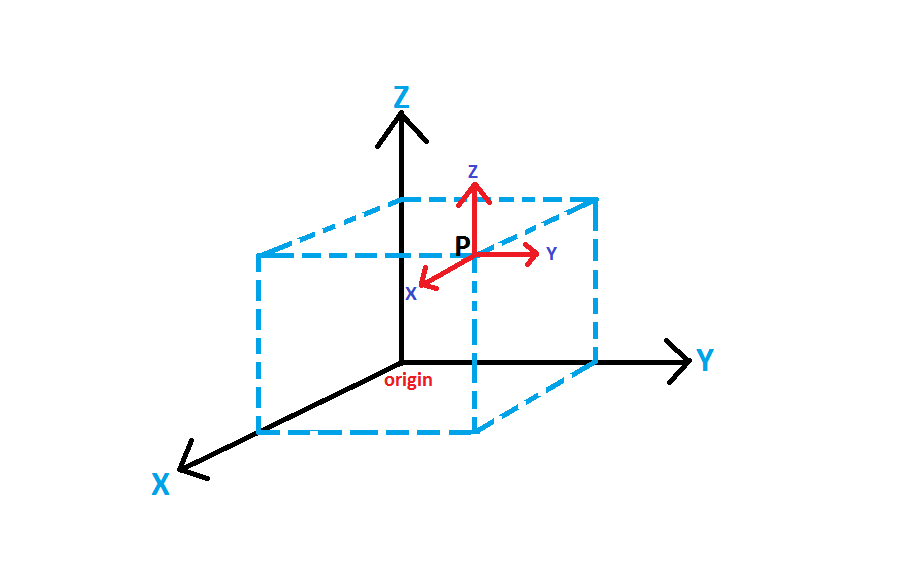
\includegraphics[width=1\linewidth]{graphics/cartesian}
\caption{The Cartesian  coordinate system}
\end{figure}

Imagine if we have a three-dimensional unbound space, like a box, the three axes will be the three edges of the box x, y, and z in the sequence x to y to z. The coordinate of a point P in the {Cartesian}\footnote{The adjective \textgravedbl{Cartesian}\textacutedbl refers to the French mathematician and philosopher Rene Descartes (1596 - 1650), born in France, he published this idea in 1637, seventeenth century. He is considered the father of modern philosophy. Many other coordinate systems have been developed since Descartes, such as the polar, cylindrical and spherical coordinates.} coordinate system can be written as $\boldsymbol{P}(x, y, z)$.The \index{right-handed coordinate system} is the convention we follow when defining the axis.
\begin{figure}[h]
\centering
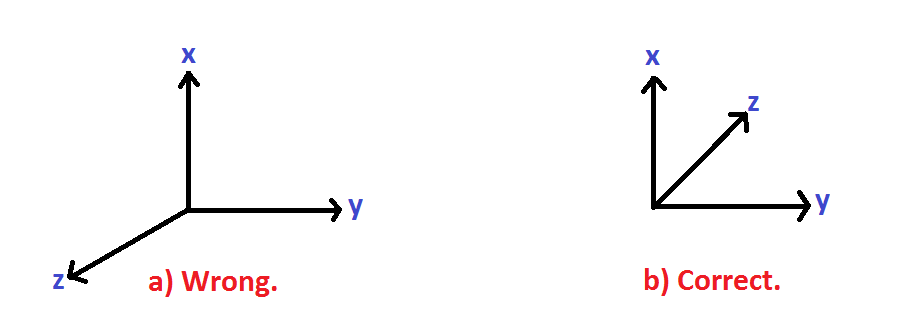
\includegraphics[width=1\linewidth]{graphics/righthand}
\caption{The right-hand coordinate system}
\end{figure}

By following the \textbf{right-hand convention}, if we point the fingers of the right hand going from X to Y, then the thumb points in the \textbf{positive} Z direction. Note that the right-hand fingers wrapped around an object shows the rotation from X to Y by the curled fingers wrapped around the object. This is X rotating towards Y to get the position Z ( thumb pointing up), that is, $\bar{X} \times \bar{Y} = \bar{Z}$; assume  $\bar{X}$ is a vector in the x direction, $\bar{Y}$ is a vector in the y direction and $\bar{Z}$ is a vector in the z-direction.

If the curl of the right-hand goes from Y to Z, the thumb will point in the direction of x or $\bar{Y} \times \bar{Z} = \bar{X}$ in vector notation form.

If the fingers curl from $\bar{Z}$ to $\bar{X}$, the thumb should point in the direction of $\bar{Y}$. The right-hand convention will enable us to resolve some ambiguity in finding the direction of the \index{vectors}, so in this case, we visualize the three-dimensional space as a box and apply the right-hand convention. As we can see here if we take a horizontal plane which is XY, you get your right-hand fingers curled from X to Y on this plane, the thumb will point upward to the Z direction. At location P for instance, we can define a vector which is represented by the arrows shown at P.

The three \index{vectors} $\mathbf{\bar{X}, \bar{Y}, \bar{Z}}$ are called the components of vector P at the location usually pointing in the three coordinate axes. Hence for any vector in space, we have the component along the x direction, along the y direction and the z direction so that any vector in space can be represented by a set of three elements. We require a lot of imagination to visualise a vector that can be the electric or magnetic field in three-dimensional space. We can write these expressions mathematically, but ultimately, it is required for one to visualize these in three-dimensional space in order to make the study of electromagnetic waves more interesting to us. The idea of visualizing the vectors in three-dimensional space is to get a physical feel for the vectors and then the problem is solved. The Cartesian coordinate system is the simplest coordinate system and the important feature of this system is that no matter where you go in space, the direction of vector P along the x, y, and z directions remains the same. This means that if we go along the Y axis, the X axis remains the same and perpendicular to the Y axis at any point in space. This may not be true for other coordinate systems, so we will write down the vector relationship for the Cartesian coordinate system since it is the coordinate system that is very easy to visualize. 

\subsection{Cylindrical coordinate system}    
\begin{figure}[h]
\centering
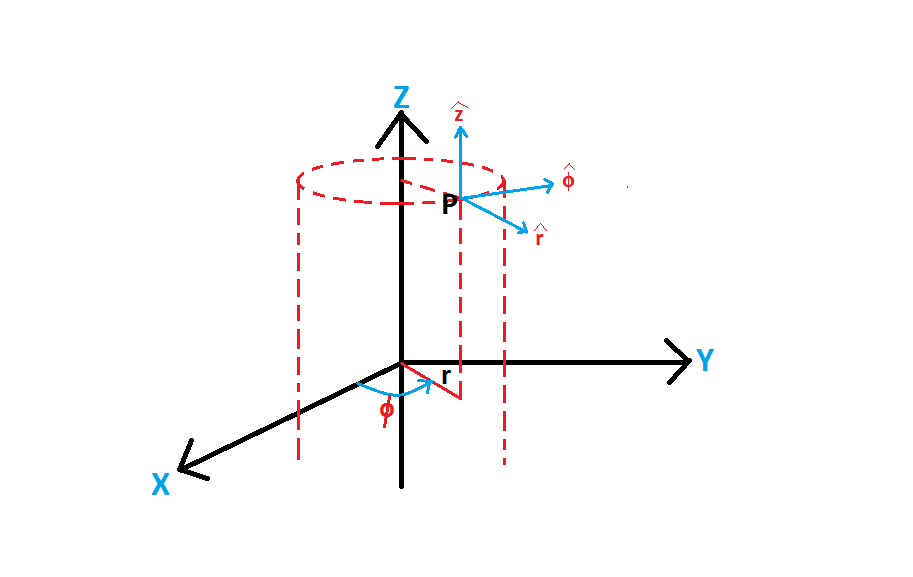
\includegraphics[width=1\linewidth]{graphics/cylindrical}
\caption{The cylindrical coordinate system}
\end{figure} 

Imagine a three-dimensional space like a cylinder, with z as the axis of the cylinder, then if we write the same cartesian coordinate x, y, z, the plane passing through XY will be perpendicular to the axis of the cylinder. The point P has a radius r, if we draw a perpendicular line from P to meet the XY plane, to make distance r, the angle that this radius vector makes with the x-axis is $\phi$. The distance we travel from the origin to meet P along the axis of the cylinder is the z point, so we have got a coordinate system with a sequence $( r, \phi, z)$. Again we follow the right-hand coordinate system, so if we have a vector, then with fingers pointed from r to $\phi $ (curling from r to $\phi$), we must get z direction and if we point from $\phi$ to z, we get r direction and so on.

\subsubsection*{ How do we define $\phi$ direction?} 
An arrow pointing in the direction of z gives the Z vector. Similarly, a vector pointing in the radius vector r outward from the origin is the r vector. The $\phi$ vector is that which is tangential to the surface of the cylinder which is passing through point P. Here we can see the relationship between the Cartesian coordinate system and the cylindrical coordinate system. The geometry of the problem determines the choice of the coordinate system to be used in the analysis of the problem. This means that we use the rectangular coordinate system for rectangular geometry, and the cylindrical coordinate system will be applied to cylindrical geometry (found in coaxial cable, optical fibre, circular waveguide, or many other structures where the geometry looks more like a cylinder).  We can analyse the problem in any coordinate system we choose, but it is easier to work in a coordinate system that is closer to the geometry of the problem, that is why when we do analysis, we first choose the appropriate coordinate system and then solve the problem of electromagnetics in that coordinate system.

The one thing we note in the cylindrical coordinate system compared to the Cartesian coordinate system is that in the Cartesian coordinate system, the direction of the x,y, and z coordinate remains the same everywhere in space no matter where the point moves, the X always orient in the same direction physically. However, in the cylindrical coordinate system, the $\hat{z}$ vector is always in the same direction no matter where you are in space but the $\hat{r}$ and $\hat{\phi}$ vector will keep changing direction as we go to different locations or points in space.

\subsection{Spherical coordinate system}
\begin{figure}[h]
\centering
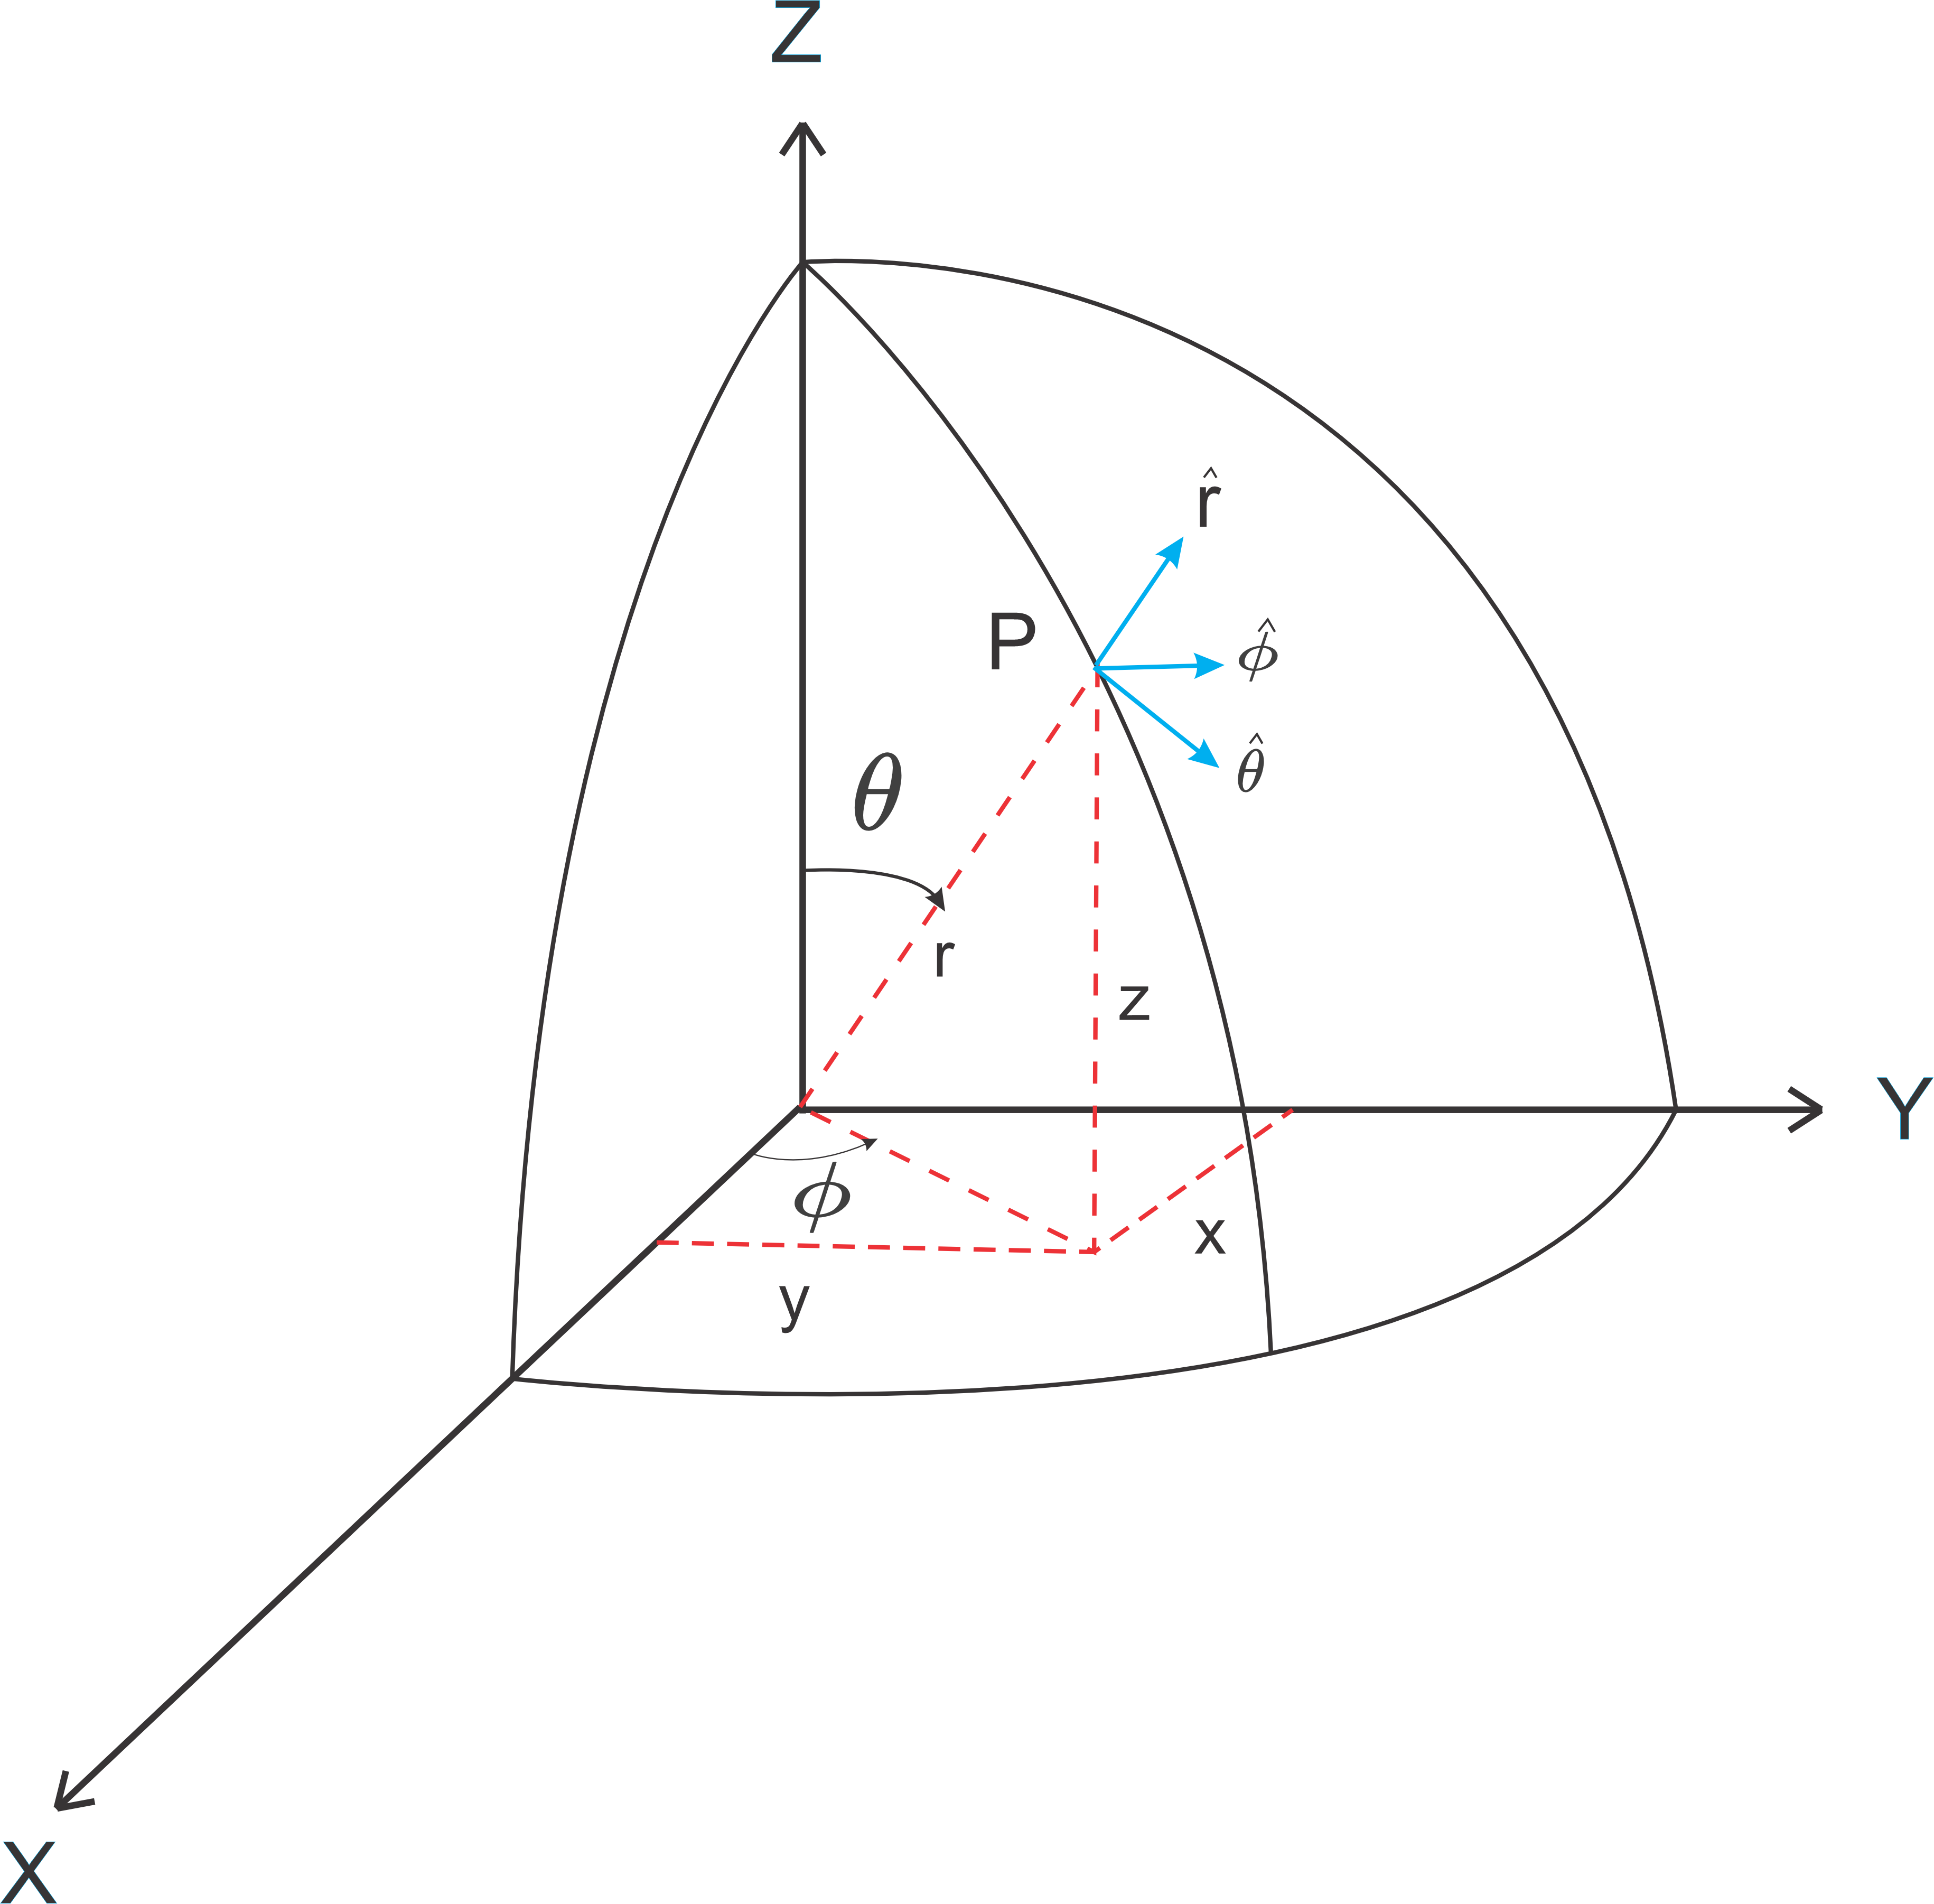
\includegraphics[width=1\linewidth]{graphics/spherical1}
\caption{The spherical  coordinate system}
\end{figure}

In this coordinate system, the three-dimensional space is imagined as a big sphere. We shall consider an octant of the sphere, with a point P marked on the surface of the sphere. P can be represented in terms of three quantities viz the radial distance of point P from origin r, the angle $\phi$ made by a line projected on the XY plane from P with the X axis, the angle $\theta$ made by a tangent to the surface in the vertical plane passing through P and this is the angle the radius vector makes with the Z axis. In this coordinate system, the point P is represented as $(r,\theta, \phi)$ in that sequence. The $r$ represents the radius vector which is the distance from the origin; $\theta$ is the angle which is measured from the z-axis to the radius vector; $\phi$ is the angle which is measured from the x-axis to the projection of the radius vector on the XY plane.

In a spherical coordinate system, the point is defined by radial distance and two angles compared to the Cartesian or cylindrical coordinate systems. In the cartesian coordinate system, the location was defined by three distances (x,y,z) but in the cylindrical coordinate system, it was defined by two distances (r,z) and one angle $\phi$.

Using the right-hand convention; if the fingers curl from r to $\theta$, then the thumb must point in the positive $\phi$ direction, if the fingers curl from $\theta$ to $\phi$, then the thumb must point in the direction of $\hat{r}$. For the spherical coordinate system, point P has $\hat{r}$ radially pointing outward and normal to the surface of the sphere; if we take an angle $\theta$ and draw a tangent passing through P at that angle, going away from $\theta$, that is, the positive direction of vector $\theta$. The right-hand rule must be followed when developing a coordinate system because when we do vector analysis, we assume that certain conventions like the right-hand convention are being applied. The figures above show how the coordinate axes are drawn when the right-hand convention is followed.

The spherical coordinate system has a special property, that is when the point called origin is defined, all measurements can be taken from there. In the Cartesian coordinate system, you can shift the origin anywhere in space whereas in the cylindrical coordinate system, the cylindrical axis line is defined and all measurements are taken from there. So whenever we have a problem like an antenna kind of problem, where we have a source of energy sending out electromagnetic waves and this source is more like a localized point or region in space, then we use the spherical coordinate system for this problem. For a problem where the energy is going to flow along the length of the structure (structures like coaxial cable, waveguide or transmission line), the cylindrical coordinate system is more appropriate or then in some general cases, the Cartesian coordinate system will be the best if we are considering a closed structure like a closed box like a resonator or a cavity. Let's go to the basic definition of vectors and their operators since we have learnt about coordinate systems. 

\section{Vector analysis}

A vector is made up of a set of three components, so any vector can be represented by three components say (a,b,c) irrespective of the coordinate system we are using. Mathematically, this description of a vector is enough. However, when we go to the solution of physical problems of electromagnetic waves, we would like to visualize these vectors in three-dimensional space even though this is abstract. Electric field and magnetic field are very abstract concepts because we do not know how to visualize these quantities, so we have to give some physical picture of these vectors by representing three components (a,b,c).\textbf{The most commonly used convention for this is to represent a vector like an arrow}, the arrow is represented with a head and a tail. The arrow direction shows the direction of the vector and the length of the arrow is the magnitude of the vector in three-dimensional space. Suppose the arrow was going away from you or coming towards you, as it goes away from us, we see a circle and an \textgravedbl X \textacutedbl covering the span of the circle and if it comes towards us we see a dot at the centre of the circle. In the arrow representation of a vector, the circle's size denotes the vector's magnitude, and a small circle represents the small magnitude of the vector.
\begin{figure}[h]
\centering
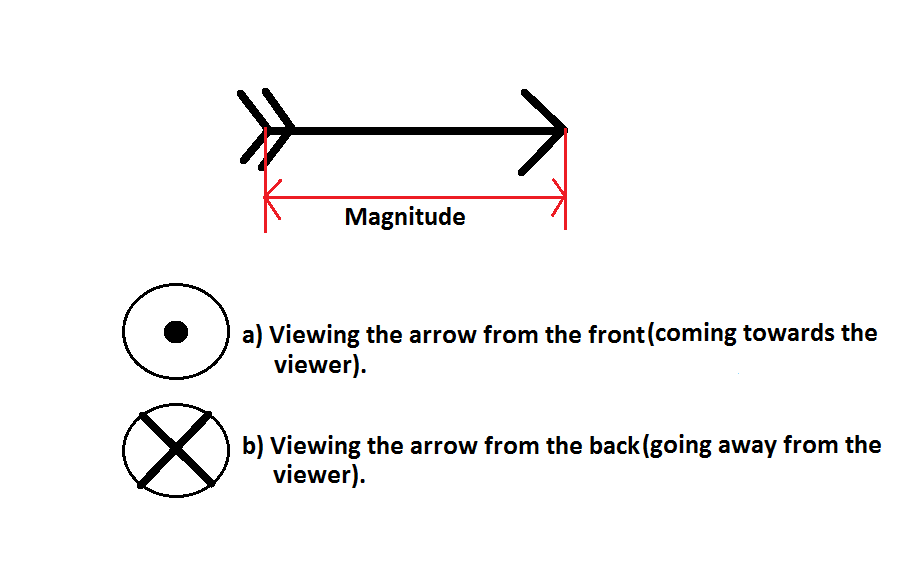
\includegraphics[width=1\linewidth]{graphics/arrowhead}
\caption{The arrowhead representation of vector}
\end{figure}

This convention shall be followed when we are visualizing three-dimensional vector fields in 3D, we see it as a distribution of these vectors or these arrows in 3D space. Abstract quantities like electric and magnetic fields will have some physical means of visualizing them and we have explained here the framework for visualizing these abstract quantities in 3D space.  

\subsection{Basic operation of vectors}
Let's say a vector A denoted as $\bar{A}$ in the Cartesian coordinate system is given as :
\begin{equation}
\bar{A} = A_{x}\hat{x} + A_{y}\hat{y} + A_{z}\hat{z} 
\end{equation}
where $\hat{x},\hat{y},\hat{z}$ are the unit vectors in the coordinate axis x,y, and z if we imagine a vector like an arrow in the direction of the X axis with unity length, then that vector is denoted as $\hat{x}$. Similarly, a vector of unit length oriented in the y direction is denoted by $\hat{y}$ and a vector of unit length oriented in the Z direction is denoted as $\hat{z}$. $A_{x}, A_{y}, A_{z}$ are called components of vector A in the x,y, and z directions respectively, so a general vector $\bar{A}$ in the three-dimensional cartesian coordinate system can be represented by the x component multiplied by the unit vector in the direction in x plus the Y component multiplied by the unit vector in the y direction, plus the z component multiplied by the unit vector in the z-direction.

Now we can define certain operations on the vector $\bar{B}$ with : 
\begin{equation}
\bar{B} = B_{x}\hat{x} + B_{y}\hat{y} + B_{z}\hat{z} 
\end{equation} 
The addition or subtraction of $\bar{A}$ and $\bar{B}$ is obtained by adding or subtracting individual components of $\bar{A}$ and $\bar{B}$.
\begin{equation}
\bar{A} + \bar{B} = (A_{x} + B_{x} )\hat{x} + (A_{y} + B_{y})\hat{y} +(A_{z} + B{z})\hat{z} 
\end{equation}
\begin{equation}
\bar{A} - \bar{B} = (A_{x} - B_{x} )\hat{x} + (A_{y} - B_{y})\hat{y} +(A_{z} - B{z})\hat{z}
\end{equation}
or in general form,
\begin{equation}
\bar{A} \pm \bar{B} = (A_{x} \pm B_{x} )\hat{x} + (A_{y} \pm B_{y})\hat{y} +(A_{z} \pm B{z})\hat{z}
\end{equation}
Another important operation these two vectors can perform is the multiplication operation. Two product operations are defined for vector quantities: a \index{scalar product} and a \index{vector product}.

\subsection{Scalar product or dot product}
\begin{equation}
\bar{A}\cdot\bar{B} = A_{x}\cdot B_{x} + A_{y}\cdot B_{y} + A_{z}\cdot B{z} 
\end{equation}
The dot product of two vectors $\bar{A}$ and $\bar{B}$ is a scalar quantity which is the sum of the product of the components of the two vectors. This is the reason it is called the \index{scalar product} of two vectors.
\subsection{Vector or cross product}

\begin{dmath*}
\bar{A} \times \bar{B} = 
\begin{vmatrix}
\hat{x} & \hat{y} & \hat{z}\\
A_{x} & A_{y} & A_{z} \\
B_{x} & B_{y} & B_{z} 
\end{vmatrix}
\end{dmath*}
We solve the determinant to get 
\begin{dmath}
\bar{A} \times \bar{B} = (A_{y}B_{z} - A_{z}B_{y})\hat{x} - (A_{x}B_{z} - A_{z}B_{x})\hat{y} + (A_{x}B_{y} - A_{y}B_{x})\hat{z}
\end{dmath}
This is called a \index{vector product} because it gives another vector. We can see that $\bar{A}.\bar{B} = \bar{B}.\bar{A} $ for the \index{scalar product}, the order does not matter but $\bar{A} \times \bar{B} \neq \bar{B} \times \bar{A}$, the magnitude of the vector remains the same but the vector $\bar{A} \times \bar{B}$ is in the opposite direction of $\bar{B} \times \bar{A}$. $\bar{A} \times \bar{B}$ represents a vector which is perpendicular to the plane containing the vector $\bar{A}$ and $\bar{B}$ if $\bar{A}$ and $\bar{B}$ were represented by two arrows, consider a plane passing through these two arrows, then the cross product vector will be a vector perpendicular to these two arrows (as shown in figure 16.6 below).

\begin{figure}[h]
\centering
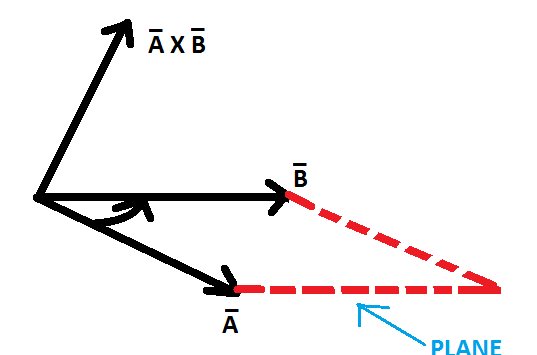
\includegraphics[width=.7\linewidth]{graphics/vector}
\caption{The representation of the cross product; $\bar{A} \times \bar{B}$ represents a vector which is perpendicular to the plane containing the vector $\bar{A}$ and $\bar{B}$. $\bar{A}$ and $\bar{B}$ are represented by two arrows, the cross-product vector will be a vector perpendicular to these two arrows.}
\end{figure}

The question is how do we know the direction of the arrow which is the cross product? With the fingers curling from $\bar{A}$ to $\bar{B}$, the direction of the thumb shows the direction of the arrow of the vector $\bar{A} \times \bar{B}$, interchanging to $\bar{B} \times \bar{A}$, the fingers will go from $\bar{B}$ to $\bar{A}$ and the direction of the thumb will be opposite so that the magnitude of the vector will remain the same, but the direction changes. These are the two important operations of vectors which we will encounter when we go to the analysis of electromagnetic waves. We require two operators on the vectors which are the differential operators. Consider a field which is a vector quantity, and at every location in space, we define this quantity which is a vector quantity. So I go to space at any point and measure it. This quantity will have magnitude at that location and this quantity will have orientation if you imagine the vector like an arrow. Let us say we have a quantity like a velocity distribution, let's say air velocity in a medium, if we go around this medium, at every location if we measure the velocity of the wind, and find out in which direction the wind is flowing, you will get the direction of the wind. So we know the extent of the wind movement and the direction in which the wind is moving. These two quantities together can be put in the form of an arrow. The extent of the wind movement is denoted as the length of the vector, and the direction in which the wind was flowing, which can be shown by the arrow. At every location, we have this quantity which is the velocity of air around that medium which can be denoted by a vector. Similarly, let's say we have a flow of some liquid, if we go to various locations, we again have a quantity which is a measure of the rate of flow of liquid at a point and if we know the direction the fluid is flowing, we again represent it with an arrow in that location. A vector field (electric field, magnetic field) is a quantity which can be represented by its strength and also its direction. In 3D space, the vector fields will be of different magnitudes and also they will have different orientations. Assuming we have a scalar field like temperature variation, we measure the variation of temperature in different directions. Suppose we take temperature variation right above the surface of the earth, we must note that temperature drop is more at a higher altitude. Along the horizontal direction, the temperature variation is almost negligible, if we travel a distance of 100 km on the earth's surface, the temperature will not vary significantly but 100 km above the surface of the earth, the temperature variation will be significant by about 40 or 50 degrees. Although temperature quantity is a scalar, its variation depends on direction, it does not have much variation in the horizontal direction but it has significant variation in the vertical direction. A scalar quantity with three dimensions can have a significant variation in different directions, the variation is a vector quantity, so we define a differential operator called the \textbf{gradient operator}. The gradient operator is used for the scalar field and the outcome of this is a vector quantity.

Let f be a function of x, y and z i.e f(x,y,z) the gradient of the scalar function f(x,y,z) represents the maximum rate of change of this function with respect to 3D space if we find the rate of change of the function in three-dimensional space x,y,z, then we find out the direction in which the function is changing maximally. The vector of the rate of change of the function f is called the gradient vector which is defined by a \index{del operator} $\nabla$
\begin{equation}
\nabla = \frac{\partial}{\partial x}\hat{x} + \frac{\partial}{\partial y}\hat{y} + \frac{\partial}{\partial z}\hat{z}
\end{equation} 
Equation 16.8 is a differential operator acting on a scalar function to give a vector. The gradient of a scalar field is 
\begin{equation}
\nabla f = \frac{\partial f}{\partial x}\hat{x} + \frac{\partial f}{\partial y}\hat{y} + \frac{\partial f}{\partial z}\hat{z}
\end{equation} 
From equation 16.9,
\begin{equation*}
\frac{\partial f}{\partial x}, \frac{\partial f}{\partial y}, \frac{\partial f}{\partial z}
\end{equation*}
It tells how far the scalar field f travels in the x, y and z directions respectively. To find out the \index{del operator} on the scalar function, we find out the rate of change of these quantities with respect to the three-dimensional space and this is the expression for the Cartesian coordinate system.
\begin{equation}
\bar{F}  =  F_{x}\hat{x} + F_{y}\hat{y} + F_{z}\hat{z}  =   \bar{F}(x,y,z)
\end{equation}
$F_{x}, F_{y}, F_{z}$ is a scalar quantity in terms of x, y and z. Now we can define the differential operators which are
\begin{enumerate}[(i)]
\item \textbf{Divergence operator} which is like dot product of the \index{del operator} and the function $\bar{F}$ i.e $\nabla.\overrightarrow{F}$ gives
\begin{equation}
\nabla.\bar{F} = \frac{\partial F_{x}}{\partial x} + \frac{\partial F_{y}}{\partial y} + \frac{\partial F_{z}}{\partial z}
\end{equation}
\item \textbf{The cross product} of $\nabla$ and $\bar{F}$ i.e $\nabla \times \bar{F}$ called the curl of vector
\begin{dmath*}
\bar{F} = \nabla \times \bar{F} = 
\begin{vmatrix}
\hat{x} & \hat{y} & \hat{z}\\
\frac{\partial}{\partial x} & \frac{\partial}{\partial y} & \frac{\partial}{\partial z}\\
F_{x} & F_{y} & F_{z}
\end{vmatrix}
\end{dmath*}
The curl of a vector is a vector quantity whereas the divergence of a vector is a scalar quantity. Next, we will get the physical feel of these quantities of divergence and curl. It will become obvious if we want to capture those physical effects, then the appropriate concepts will be divergence and curls. Divergence and curl are the basic concepts applied to solve electromagnetic problems.
\end{enumerate}
\section{Exercises}
\begin{ExerciseList}
	\Exercise[label={ex161}] 
	In the description of a vector using arrow notation, the length of the arrow may represent what property of the vector?
	
	\Exercise[label={ex162}] 
	What is the relationship between the direction of the cross product of vectors and the plane of vectors?
	
	\Exercise[label={ex163}] 
	The outcome of the gradient of a scalar field is what quantity?
	
	\Exercise[label={ex164}] 
	Contrast the outcome of the divergence of a vector field and the curl of a vector field. 
	
	\Exercise[label={ex165}] 
	What are the basic importance of scalar and \index{vector products} in the basic concept applied to solve electromagnetic problems?  
	
	\Exercise[label={ex166}] 
	If you switch on a torch and point it in any direction, what happens to the rays of light?
	
	\Exercise[label={ex167}] 
	If $\bar{A} = 2\hat{x} + 3\hat{z}$ and $\bar{B} = 4\hat{x} - \hat{y} + 3\hat{z}$, find: 
	(i) $\bar{A} \times \bar{B}$
	(ii) $\bar{B} \times \bar{A}$  
	\Answer
	(i). 3$\hat{x}$+6$\hat{y}$-2$\hat{z}$
	(ii).-3$\hat{x}$-6$\hat{y}$+2$\hat{z}$
	\Exercise[label={ex168}] 
	What is the gradient of the given scalar field: $F = \frac{\cos(5x)}{y}$
	\Answer
	$\nabla F = \frac{-5\sin(5x)}{y}\hat{x} - \frac{\cos(5x)}{y^2}\hat{y}$


	\Exercise[label={ex169}] 
	A field is said to contain only magnitude, and we need to perform an operation on this field to produce a vector field. Carry out this analysis on this given field: $T = x^2yz^3 + xy^2z^2$.
	\Answer
	$\nabla T= (2xyz^3+y^2z^2)\hat{x}+(x^2z^3+2xyz^2)\hat{y}+(3x^2yz^2+2xy^2z)\hat{z}$

	\Exercise[label={ex1610}] 
	Check if the fields given below have a tendency to curl or diverge and write a brief discussion on what actually happens.
	$\bar{P}$ = x$\sin$(2y)$\hat{x}$, $\bar{Q}$ = $e^{y}$$\cos$(z)$\hat{x}$ + $\sinh(x)$$\hat{y}$.
	\Answer
	(i).$\nabla$$\dot{\bar{P}}$=$\sin(2y)$$\hat{z}$
	(ii).$\nabla$$\cross$$\bar{P}$= $2x\cos(2y)$$\hat{z}$
	(iii).$\nabla$$\dot{\bar{Q}}$ = 0
	(iv).$\nabla$$\cross$$\bar{Q}$= -$e^{y}$$\sin(z)$$\hat{y}$ + ($\cosh(x)$ - $ye^{y}$$\cos(z)$)$\hat{z}$
\end{ExerciseList}